\documentclass[../main.tex]{subfiles}
\begin{document}

\section{Empirical Application Details}
\label{app:application-details}

This appendix documents the ten empirical audits summarized in \autoref{sec:application}. Each application fixes one target estimand, validates its full-sample coefficient, constructs an MIS-compatible linear representation, and searches deletion sets in both directions of coefficient movement. The default deletion budget is
\[
k=1,\ldots,\lfloor 0.05N\rfloor,
\]
subject to paper-specific feasibility restrictions. Every selected deletion set is subsequently evaluated using the corresponding paper-specific estimator. The reported paths therefore use exact feasible refits for the target coefficient.

For comparability across applications, let
\[
R_k
=
\frac{\widehat{\beta}_{(-S_k)}}{\widehat{\beta}_0},
\]
where \(\widehat{\beta}_0\) is the validated full-sample coefficient and
\(\widehat{\beta}_{(-S_k)}\) is the exact refitted coefficient after deleting the selected size-\(k\) set. A \(50\%\) attenuation is reached when \(R_k\leq0.5\), a \(50\%\) amplification when \(R_k\geq1.5\), and a zero crossing when \(R_k\leq0\). Amplification and attenuation are defined relative to the direction of the original coefficient, so these thresholds remain comparable for positive and negative baseline estimates.

The study-specific figures plot
\[
\Delta\beta_k
=
\widehat{\beta}_{(-S_k)}-\widehat{\beta}_0
\]
against the number of deleted observations. The upper horizontal axis reports the corresponding share of the estimation sample. The solid horizontal reference denotes no coefficient change, while the dashed horizontal reference denotes the change required for the refitted coefficient to equal zero. A vertical dotted line is shown when a zero crossing is reached within the audit budget.


\subsection{Study 01: Mobile Money}
\label{app:application-01}

The first audit considers the primary capital outcome in \emph{Resisting Social Pressure in the Household Using Mobile Money}. The target is the coefficient on Mobile Disburse, denoted by \texttt{treatment3}, in the paper's fixed-effects OLS specification. The regression includes baseline capital, the alternative treatment indicator, and randomization-strata fixed effects. The validated estimation sample contains \(N=2{,}639\) observations, and the full-sample target coefficient is
\[
\widehat{\beta}_0=69.2072.
\]
The MIS representation replaces the absorbed fixed effects with explicit indicators and reproduces the target coefficient to numerical precision. Exact deletion refits then use the original fixed-effects estimator.

The coefficient responds to deletions well below the common \(5\%\) budget. A \(50\%\) amplification is first attained after deleting \(13\) observations, approximately \(0.49\%\) of the estimation sample, while a \(50\%\) attenuation is attained after \(14\) deletions, approximately \(0.53\%\). The first zero crossing occurs at \(k=41\), corresponding to approximately \(1.55\%\) of the sample. The selected capital coefficient is therefore sensitive to relatively small feasible deletion sets in both directions.

\begin{figure}[htbp]
\centering
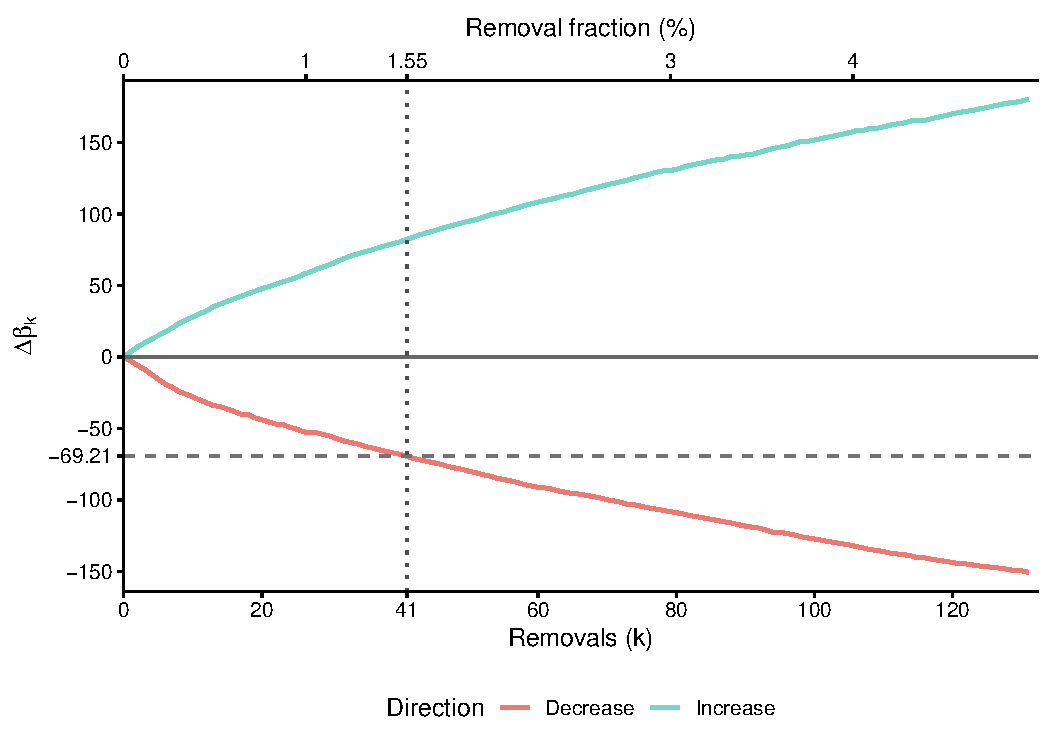
\includegraphics[width=0.88\textwidth]{../../application/01_RSPitHUMM/fig_mis_audit.pdf}
\caption{Observation-sensitivity paths for the Mobile Disburse coefficient in the mobile-money application. The paths report exact fixed-effects OLS refits after each selected deletion set.}
\label{fig:app01-mis-audit}
\end{figure}


\subsection{Study 02: Vaccine Delivery}
\label{app:application-02}

The second audit considers Table 1, column (1), of \emph{Last-mile delivery increases vaccine uptake in Sierra Leone}. The outcome is endline vaccination status, and the target coefficient is the door-to-door treatment indicator \texttt{treat\_dtd}. The alternative treatment arm, \texttt{treat\_small}, remains in the regression as a nuisance treatment regressor. The validated fixed-effects estimation sample contains \(N=12{,}096\) observations, with
\[
\widehat{\beta}_0=0.2935.
\]
The search representation uses explicit fixed-effect indicators, while exact deletion refits preserve the paper's fixed-effects estimator. Community-level clustering affects inference but does not change the point coefficient targeted by the audit.

This coefficient is comparatively stable over the searched deletion range. A \(50\%\) attenuation is first reached after deleting \(505\) observations, approximately \(4.17\%\) of the estimation sample. A \(50\%\) amplification is not reached, and the coefficient does not cross zero within the maximum audited deletion share of approximately \(5\%\). The result therefore remains positive throughout the prespecified audit budget.

\begin{figure}[htbp]
\centering
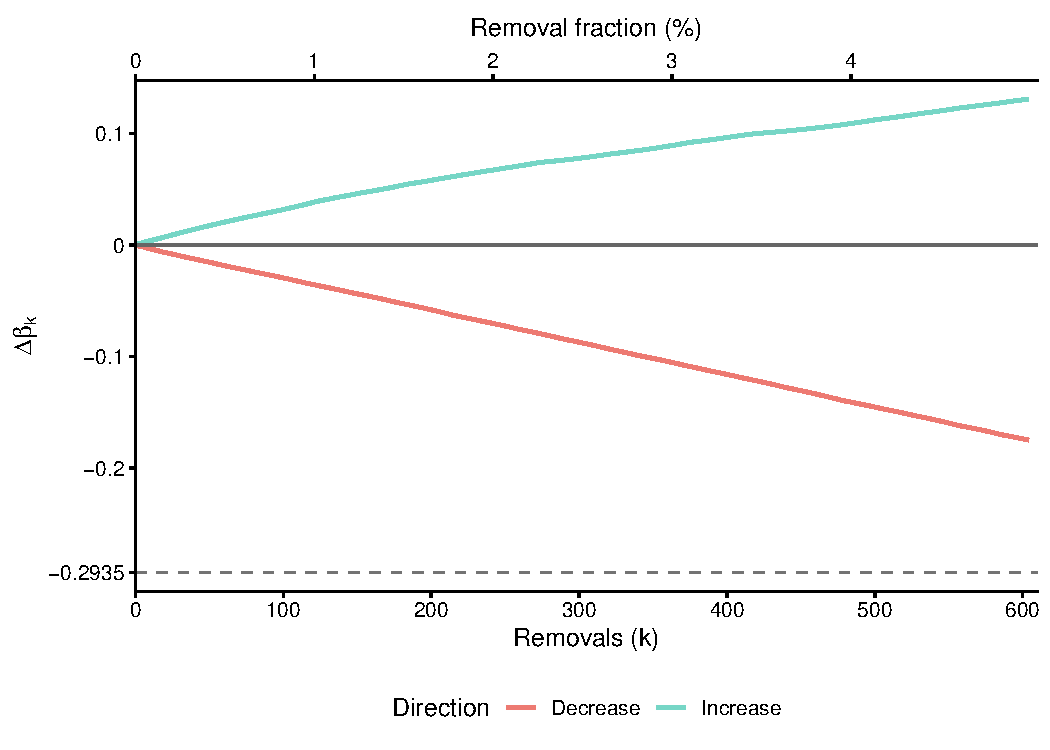
\includegraphics[width=0.88\textwidth]{../../application/02_LMDIVUiSL/fig_mis_audit.pdf}
\caption{Observation-sensitivity paths for the door-to-door vaccination coefficient in the vaccine-delivery application.}
\label{fig:app02-mis-audit}
\end{figure}


\subsection{Study 03: Self-Esteem}
\label{app:application-03}

The third audit examines the first-follow-up, full-sample specification from Table 5 of \emph{What's Behind Her Smile? Health, Looks, and Self-Esteem}. The outcome is standardized Rosenberg self-esteem, \texttt{sd\_rosen1}, and the target is the treatment coefficient. The preferred linear specification includes baseline self-esteem, baseline characteristics, and randomization-strata indicators. The validated sample contains \(N=634\) observations, with
\[
\widehat{\beta}_0=0.2317.
\]
Because heteroskedasticity-robust covariance estimation does not alter the OLS point estimate, the same linear specification is used for the MIS search and the exact point-estimate refits.

A \(50\%\) attenuation is attained after deleting \(16\) observations, approximately \(2.52\%\) of the sample, while a \(50\%\) amplification requires \(18\) observations, approximately \(2.84\%\). The coefficient does not cross zero within the maximum deletion budget. The audit therefore identifies substantial movement in the magnitude of the treatment coefficient without a reversal of its sign.

\begin{figure}[htbp]
\centering
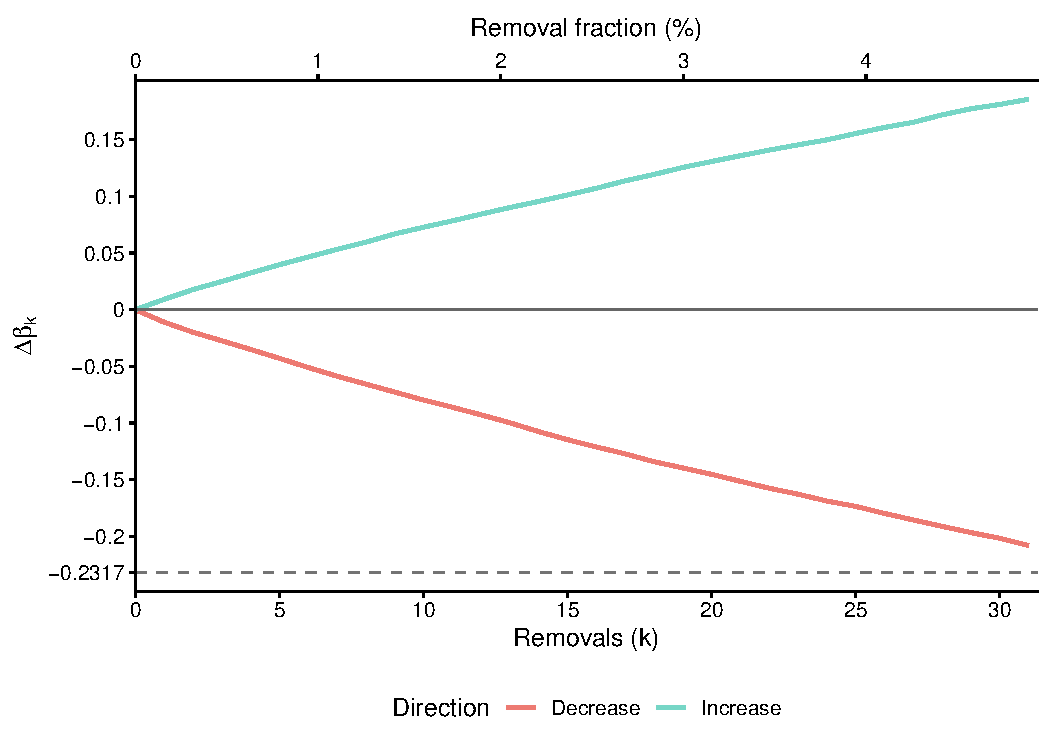
\includegraphics[width=0.88\textwidth]{../../application/03_WbHS/fig_mis_audit.pdf}
\caption{Observation-sensitivity paths for the treatment coefficient in the self-esteem application.}
\label{fig:app03-mis-audit}
\end{figure}


\subsection{Study 04: Health Information and Survival}
\label{app:application-04}

The fourth audit considers the survival analysis in \emph{Surviving Bad News: Health Information without Treatment Options}. The target is the coefficient on \texttt{learnhivpos} in the reported OLS companion specification for survival in 2018. The regression retains the coefficient for learning HIV-negative status and controls for HIV status, sex, age, age squared, and regional indicators. The validated estimation sample contains \(N=2{,}332\) observations, with
\[
\widehat{\beta}_0=-0.1566.
\]

The coefficient is sensitive to small deletion sets. A \(50\%\) amplification in the original negative direction is reached after deleting \(5\) observations, approximately \(0.21\%\) of the estimation sample, while a \(50\%\) attenuation is reached after \(9\) deletions, approximately \(0.39\%\). The coefficient first crosses zero after deleting \(17\) observations, approximately \(0.73\%\) of the sample. The audit also records non-nested transitions along the deletion paths, indicating that the composition of the selected influential set can change as \(k\) increases.

The scope of this audit is narrower than the preferred causal analysis in the original study. The paper's preferred specifications use instrumental variables and efficient linear GMM, while the current shared MIS engine is defined for a linear OLS representation. The results in this appendix therefore apply to the reported OLS companion coefficient and should not be interpreted as an MIS audit of the preferred IV/GMM causal estimate.

\begin{figure}[htbp]
\centering
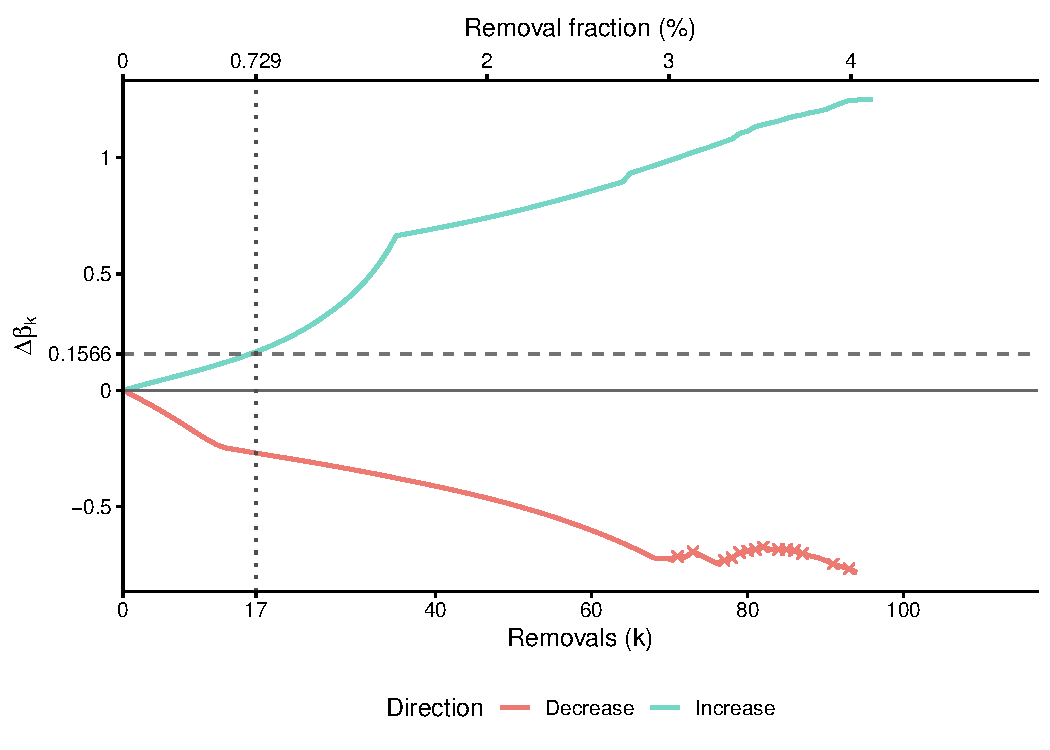
\includegraphics[width=0.88\textwidth]{../../application/04_SBN-HIWTO/fig_mis_audit.pdf}
\caption{Observation-sensitivity paths for the OLS coefficient on learning HIV-positive status in the health-information application.}
\label{fig:app04-mis-audit}
\end{figure}


\subsection{Study 05: Cash versus In-Kind Transfers}
\label{app:application-05}

The fifth audit examines aggregate food consumption in \emph{Testing Paternalism: Cash versus In-Kind Transfers}. The target is the contrast between the in-kind treatment effect and the equal-value cash treatment effect,
\[
\operatorname{ATT}(\text{In-kind})
-
\operatorname{ATT}_{EQ}(\text{Cash}).
\]
The validated analysis uses the no-village-controls specification. An algebraic reparameterization places this contrast directly on the coefficient \texttt{ik\_minus\_eq\_cash} without changing the model span, fitted values, residuals, or estimation sample. The validated sample contains \(N=10{,}985\) observations, and the baseline contrast is
\[
\widehat{\beta}_0=-0.8861.
\]

This application exhibits the smallest deletion thresholds among the ten audits. On the relevant directional paths, the \(50\%\) attenuation, \(50\%\) amplification, and zero-crossing thresholds are each attained at \(k=1\), corresponding to approximately \(0.009\%\) of the estimation sample. Different directional searches can select different observations at the same deletion size, so these thresholds should not be interpreted as requiring the same single observation.

The scope qualification is important. The replication retains unresolved differences in the fully controlled aggregate-consumption specification, whereas the no-village-controls aggregate regression reproduces the relevant benchmark and is therefore used for the MIS audit. The results should consequently be interpreted as sensitivity of this validated no-village-controls contrast.

\begin{figure}[htbp]
\centering
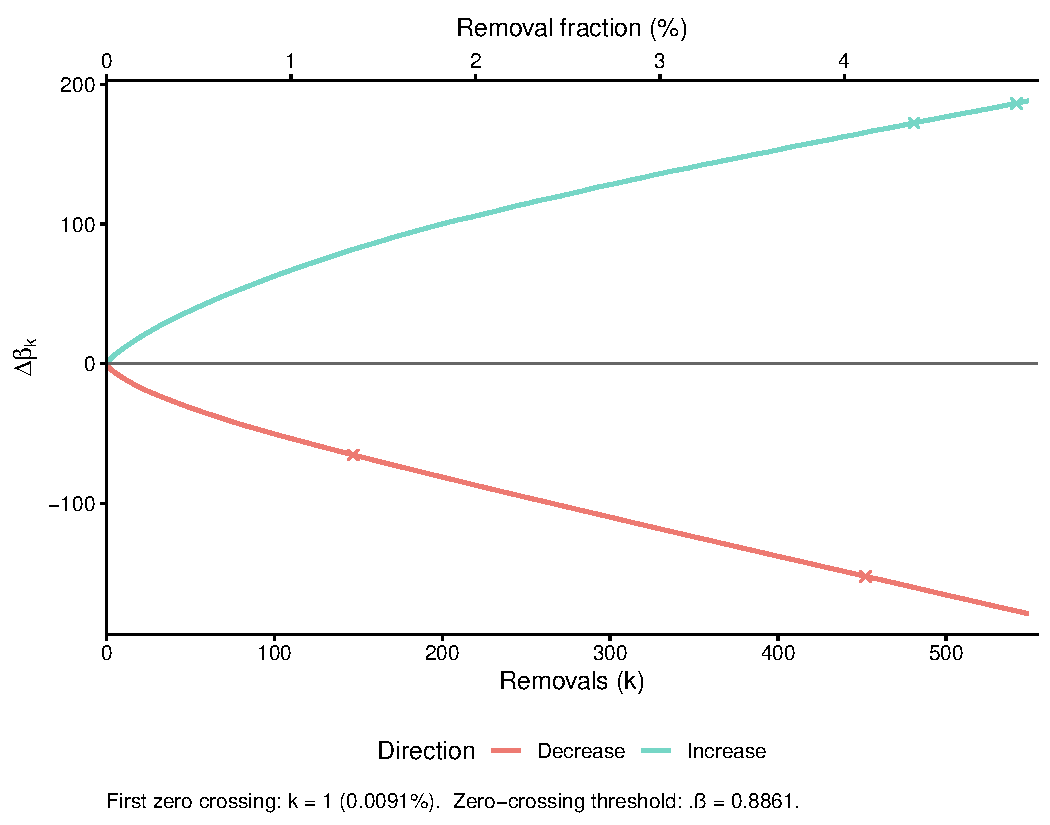
\includegraphics[width=0.88\textwidth]{../../application/05_TPCvIKT/fig_mis_audit.pdf}
\caption{Observation-sensitivity paths for the in-kind versus equal-value cash contrast in the food-consumption application.}
\label{fig:app05-mis-audit}
\end{figure}


\subsection{Study 06: Workforce Grant}
\label{app:application-06}

The sixth audit considers the main intent-to-treat employment specification in \emph{Using Household Grants to Benchmark the Cost Effectiveness of a USAID Workforce Readiness Program}. The outcome is \texttt{bn\_employed}, and the target coefficient is \texttt{treat\_HD}. The paper estimates the model by fixed-weight weighted least squares with baseline outcomes, selected controls, and randomization-block indicators. The validated sample contains \(N=1{,}770\) observations, with
\[
\widehat{\beta}_0=0.0231.
\]

The MIS search represents the fixed-weight estimator through the exact transformation
\[
y_i^*=\sqrt{w_i}y_i,
\qquad
X_i^*=\sqrt{w_i}X_i.
\]
Deleting a transformed row is therefore equivalent to deleting the corresponding original observation while holding the weights fixed. Every selected set is subsequently re-estimated with the original weighted estimator.

A \(50\%\) amplification is first attained after deleting \(4\) observations, approximately \(0.23\%\) of the sample, while a \(50\%\) attenuation occurs after \(5\) deletions, approximately \(0.28\%\). The coefficient first crosses zero at \(k=10\), corresponding to approximately \(0.56\%\) of the estimation sample. The selected employment coefficient is therefore sensitive to deletion sets containing well below one percent of the validated sample.

\begin{figure}[htbp]
\centering
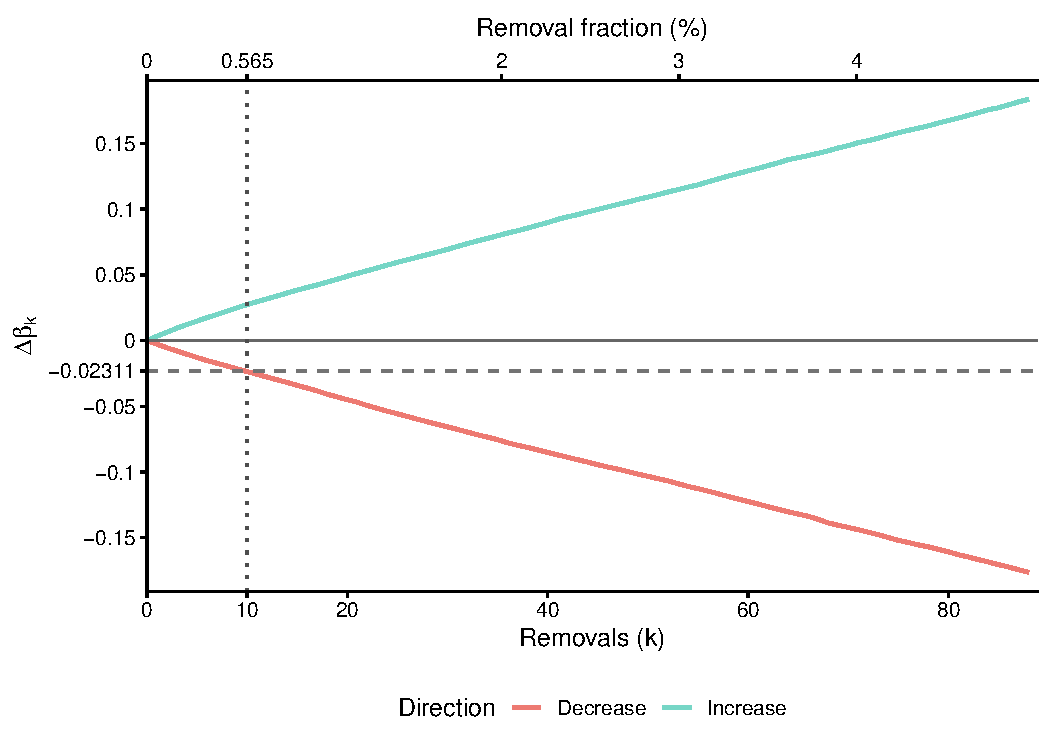
\includegraphics[width=0.88\textwidth]{../../application/06_UHGtBtCEoaUWRP/fig_mis_audit.pdf}
\caption{Observation-sensitivity paths for the target employment coefficient in the workforce-grant application.}
\label{fig:app06-mis-audit}
\end{figure}


\subsection{Study 07: Sanitation Spillovers}
\label{app:application-07}

The seventh audit examines the decision-spillover specification in Table 2 of \emph{Spillovers without Social Interactions in Urban Sanitation}. The analysis is restricted to treated households, the outcome is \texttt{signup\_all}, and the target coefficient is \texttt{neighbor\_high}. The own-subsidy variable \texttt{subsidy\_high} remains in the specification. The validated estimation sample contains \(N=3{,}757\) observations, and the baseline coefficient is
\[
\widehat{\beta}_0=-0.00976.
\]

The original specification uses post-double-selection LASSO to determine nuisance controls before estimating the target coefficient. The audit reproduces this selection step on the validated full sample and then freezes the selected controls throughout the deletion path. Re-running LASSO after each deletion would change the nuisance specification as \(k\) changes and would therefore define a different sensitivity problem. Exact deletion refits use the resulting fixed-effects OLS specification.

A \(50\%\) amplification is reached after deleting \(15\) observations, approximately \(0.40\%\) of the sample, while a \(50\%\) attenuation occurs after \(16\) deletions, approximately \(0.43\%\). The coefficient first crosses zero after \(33\) deletions, corresponding to approximately \(0.88\%\) of the estimation sample. The selected spillover coefficient is therefore sensitive within the first one percent of the deletion path.

\begin{figure}[htbp]
\centering
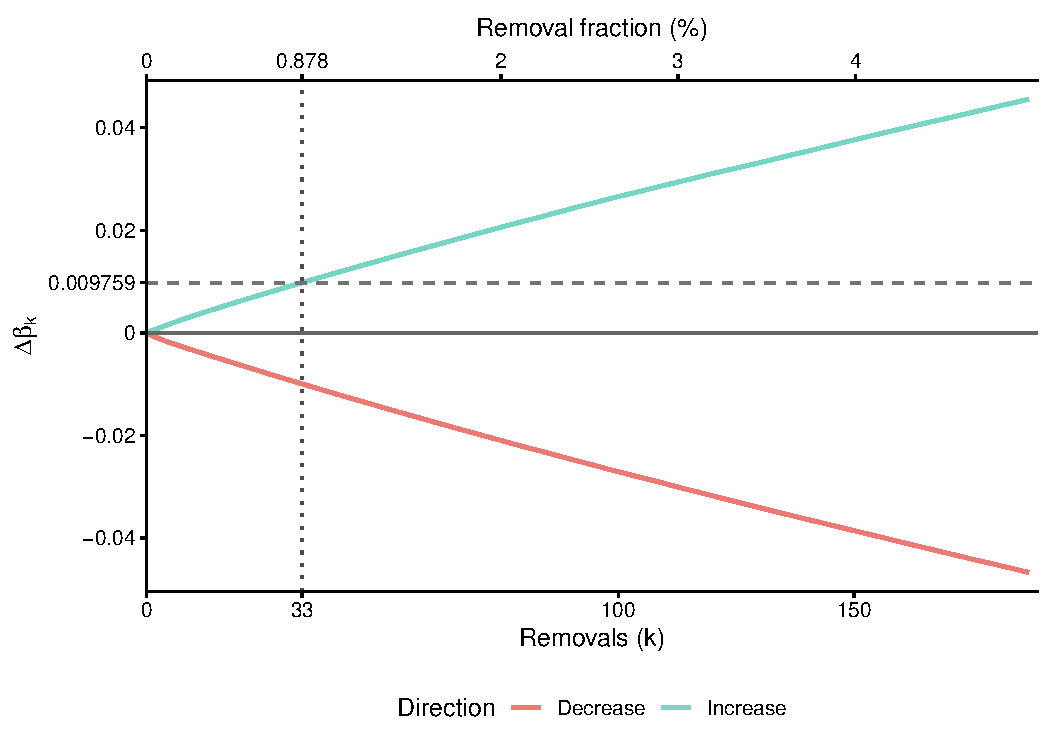
\includegraphics[width=0.88\textwidth]{../../application/07_SwSIiUS/fig_mis_audit.pdf}
\caption{Observation-sensitivity paths for the neighboring-treatment coefficient in the sanitation-spillover application.}
\label{fig:app07-mis-audit}
\end{figure}


\subsection{Study 08: Access to Finance}
\label{app:application-08}

The eighth audit considers the main firm-level specification in Table 3 of \emph{Indirect Effects of Access to Finance}. The outcome is firm log sales, \texttt{lnpart5revenue}, and the target coefficient \texttt{inter4post} measures post-treatment exposure to the share of competitors receiving access to finance. The firm's own treatment effect remains in the regression. The validated estimation sample contains \(N=8{,}612\) observations, with
\[
\widehat{\beta}_0=-0.08555.
\]

The original model contains firm fixed effects. The MIS representation uses explicit firm indicators and reproduces the target coefficient before the deletion search, while exact deletion refits use the paper-specific fixed-effects estimator. This distinction also preserves the complete validated Table 3 sample when the fixed-effects implementation removes singleton groups internally.

The target coefficient is sensitive at very small deletion fractions. A \(50\%\) attenuation is first reached after deleting \(5\) observations, approximately \(0.058\%\) of the estimation sample, and a \(50\%\) amplification is reached after \(8\) deletions, approximately \(0.093\%\). The coefficient first crosses zero after deleting \(20\) observations, or approximately \(0.23\%\) of the sample. The audit also records several non-nested transitions as the deletion budget increases, consistent with the changing influential-set structure illustrated in \autoref{fig:application-persistence}.

\begin{figure}[htbp]
\centering
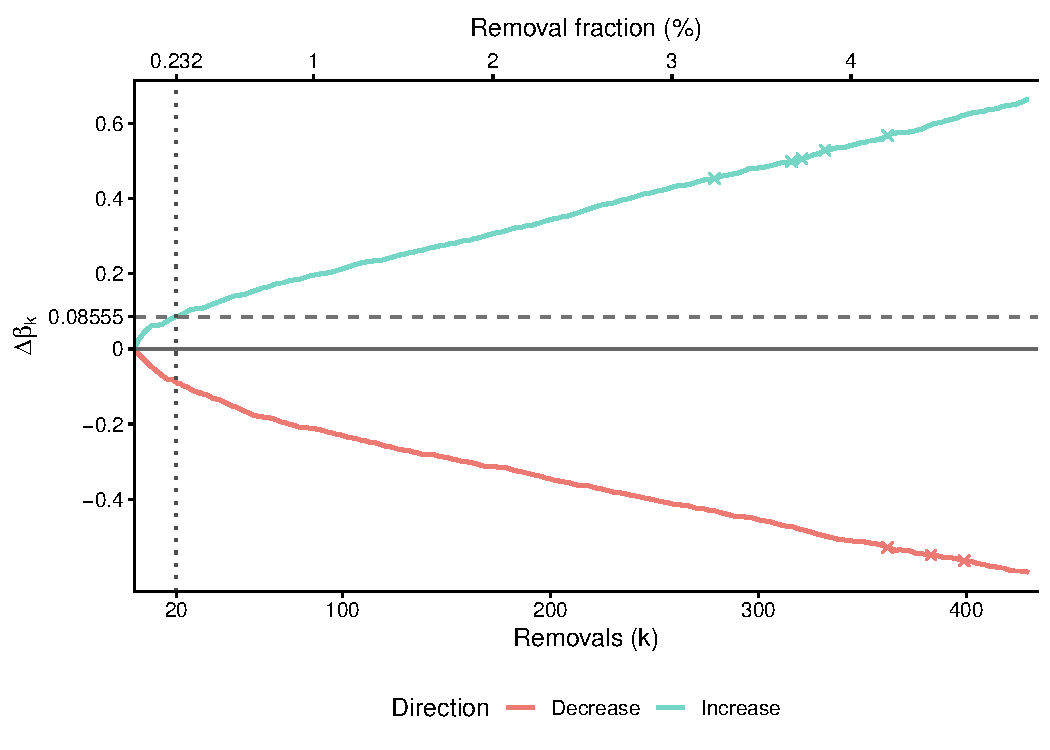
\includegraphics[width=0.88\textwidth]{../../application/08_IEoAtF/fig_mis_audit.pdf}
\caption{Observation-sensitivity paths for the competitor-treatment exposure coefficient in the access-to-finance application.}
\label{fig:app08-mis-audit}
\end{figure}


\subsection{Study 09: Immunization Nudges}
\label{app:application-09}

The ninth audit considers the post-selection pooled policy model for immunizations per dollar in \emph{Selecting the Most Effective Nudge}. The target is the pooled coefficient combining information-hub ambassadors with SMS reminders and no incentives. The validated village-month estimation sample contains \(N=7{,}370\) observations, with
\[
\widehat{\beta}_0=0.004016.
\]

The published workflow first performs variable selection and policy pooling and subsequently estimates a weighted post-selection model. The audit reconstructs the selection and pooling procedure once on the validated full sample and freezes the resulting specification throughout the deletion path. Fixed village-population weights are represented through the exact square-root-weight transformation used for Study 06, and every selected deletion set is subsequently re-estimated with the original weighted estimator.

A \(50\%\) amplification is reached after deleting \(55\) observations, approximately \(0.75\%\) of the sample. A \(50\%\) attenuation requires \(105\) observations, approximately \(1.42\%\), and the first zero crossing occurs at \(k=214\), corresponding to approximately \(2.90\%\) of the estimation sample. The audit records non-nested changes in influential-set membership as \(k\) increases. The geographic composition of the \(214\)-observation sign-reversing set is examined separately in \autoref{fig:application-spatial-concentration}.

\begin{figure}[htbp]
\centering
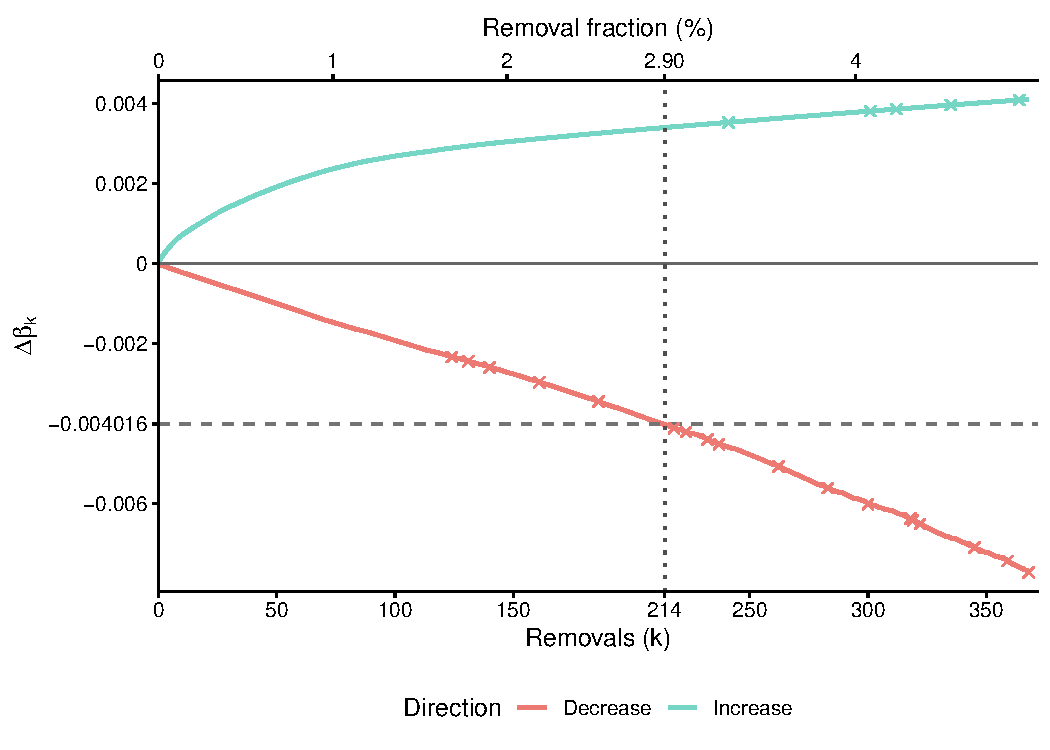
\includegraphics[width=0.88\textwidth]{../../application/09_StMEN/fig_mis_audit.pdf}
\caption{Observation-sensitivity paths for the selected pooled policy coefficient in the immunization application.}
\label{fig:app09-mis-audit}
\end{figure}


\subsection{Study 10: Electricity Information}
\label{app:application-10}

The tenth audit considers the distribution-information treatment in \emph{The Power of Information: A Survey Experiment on Public Support for Electricity Price Compensation Schemes}. The target is \texttt{T1} in the reported Table A5 linear-probability robustness model for support for the price-subsidy scheme. The other randomized information treatments remain in the regression. The validated estimation sample contains \(N=1{,}819\) observations, with
\[
\widehat{\beta}_0=-0.1168.
\]

A \(50\%\) amplification in the original negative direction is first attained after deleting \(32\) observations, approximately \(1.76\%\) of the sample. A \(50\%\) attenuation occurs after \(34\) deletions, approximately \(1.87\%\), and the coefficient crosses zero after deleting \(63\) observations, corresponding to approximately \(3.46\%\) of the estimation sample. The sign of the linear-probability estimate is therefore preserved over a larger deletion fraction than in most of the sign-reversing applications, although a reversal remains feasible within the common \(5\%\) budget.

The paper's headline specification uses an ordered-logit estimator. The shared MIS search is defined for a linear model, so the present audit uses the paper's reported linear-probability robustness specification for the same randomized treatment contrast. The results therefore characterize observation sensitivity of the Table A5 linear coefficient and should not be interpreted as a deletion audit of the headline ordered-logit estimate.

\begin{figure}[htbp]
\centering
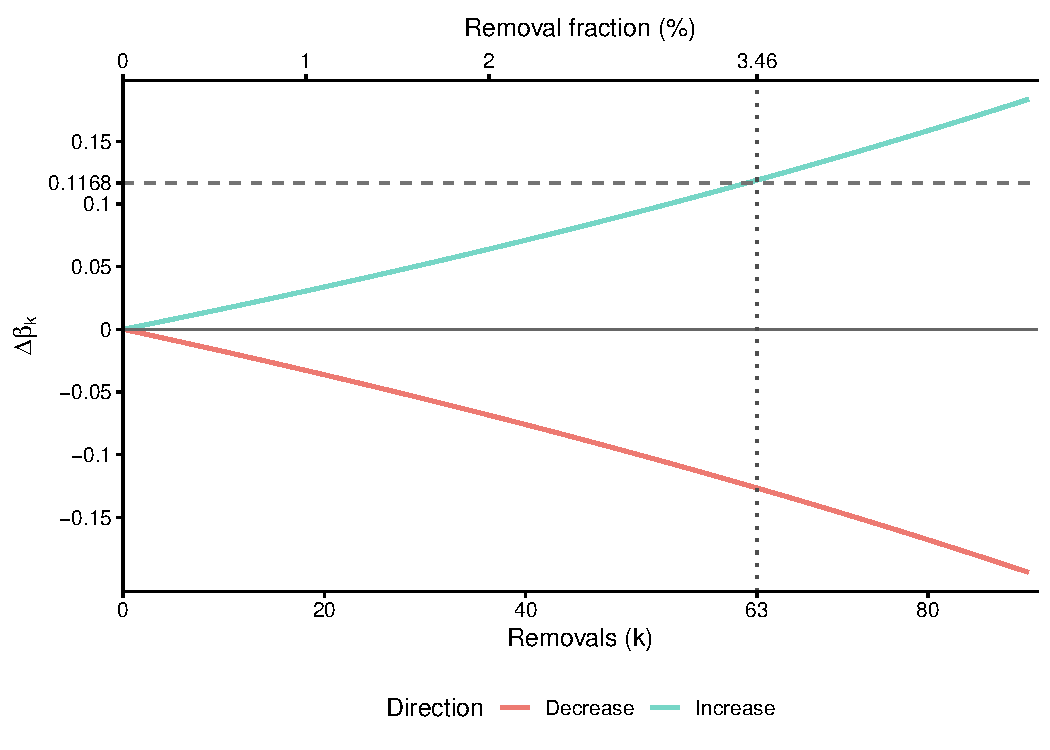
\includegraphics[width=0.88\textwidth]{../../application/10_TPoI/fig_mis_audit.pdf}
\caption{Observation-sensitivity paths for the distribution-information coefficient in the electricity-information application.}
\label{fig:app10-mis-audit}
\end{figure}


\subsection{Interpretation of the Study-Specific Audits}
\label{app:application-interpretation-summary}

The ten audits apply a common sensitivity question to paper-specific estimands whose estimation structures differ. Fixed effects are represented explicitly where required, fixed weights are handled through an exact transformed regression, and model-selection steps are frozen when repeated selection would alter the nuisance specification. Baseline equivalence is established before the deletion search in every application. The resulting paths therefore refer to explicitly defined and validated coefficients.

The study-specific results also clarify the scope of the cross-study comparison in \autoref{subsec:application-sensitivity}. A low deletion threshold establishes that a feasible small subset can induce a large change in the selected point estimate. A higher threshold indicates greater stability over the corresponding deletion range. Neither result evaluates the experimental design as a whole, and a zero crossing does not imply that every finding in the source study is similarly sensitive. The empirical application therefore treats MIS as a targeted diagnostic of finite-sample observation sensitivity.

\end{document}